\documentclass[12pt,twoside]{article}

\usepackage{a4wide}            % A4 verwenden (und ausnutzen)
\usepackage[ngerman]{babel}   % Deutsche Silbentrennung, Sonderzeichen, etc
\usepackage[utf8x]{inputenc}  % Im TeX-File Umlaute erlauben ä statt "a
\usepackage[T1]{fontenc}       % Umlaute f"ur Silbentrennung kodieren
\usepackage{ae}                % Type-1 Font verwenden
\usepackage{graphicx}          % Einbinden von PS-Graphiken
\usepackage{pstricks,pst-node} % Eigene Zeichnungen erlauben
\usepackage{fancyhdr}          % Kopfzeilen
\usepackage{url}               % URL
\pagestyle{fancyplain}

\begin{document}
\author{Tobias Harrer, Daniel Felsmann}
\title{Protokoll: Bakterienwachstum und -transformation}
\date{06.11.2012}
\maketitle
\tableofcontents
\newpage 
\section{Versuch 1: Bakterielles Wachstum}
\subsection{Einleitung}
Die Versuche der vierten Woche befassten sich zum Einen mit dem Wachstum von Bakterienkulturen der "Labor-Art" Escherichia coli K12 und zum Anderen der Transformierung von Bakterien mit Plasmid DNA. Falls die für das Bakteriumwachstum günstigen Bedingungen, also ausreichend Nährstoffe und eine Temperatur von 37°C, vorliegen, können sich Bakterien in einer Zeit von bis zu 20 Minuten durch Zellteilung verdoppeln. Dies lässt auf ein exponentielles Wachstum schließen, da sich jedes neu entstandene Bakterium wieder Teilen wird. Dieses Wachstum ist aber nach relativ kurzer Zeit durch die sich ändernden Umweltbedingungen begrenzt, wobei zum Einen die Nährstoffe nicht unbegrenzt vorhanden sind, der Bedarf allerdings exponentiell ansteigt, und sich zum Anderen auch die Stoffwechselendprodukte der Bakterien in exponentiellem Ausmaß anhäufen. Dadurch kann die Entwicklung einer Bakterien wie folgt in vier Phasen eingeteilt werden:
\begin{enumerate}
\item Lag Phase: Die Bakterien bereiten sich für die Teilung vor.
\item Log Phase: Die Bakterien teilen sich, ihre Anzahl steigt exponentiell.
\item Stationäre Phase: Durch Mangel an Nährstoffen und vermehrtem Anfallen giftiger Stoffwechselendprodukte sterben genau so viele Bakterien, wie in der selben Zeit durch Teilung neu entstehen können.
\item Death Phase: Das Verhältnis Nährstoffe zu Abfallprodukte liegt so weit rechts, dass weitere Zellteilungen nicht mehr möglich sind, viel mehr sterben jetzt mehr Zellen als neue nachgebildet werden können.
\end{enumerate}
Während der Log-Phase beträgt die Anzahl der Bakterien in der Kolonie nach n Verdopplungszeiten $A(n) = A_0 \cdot 2^{n}$, wobei $A_0$ die Anzahl der Bakterien zu Beginn, also in der \textit{Lag-Phase} darstellt. \newline
Um die Anzahl der Bakterien quantitativ bestimmen zu können, prüft man die Lichtdurchlässigkeit bei 600 nm des Nährmediums, in dem das Bakteriumwachstum stattfindet.
\subsection{Material, Methoden, Durchführung}
\textit{Benötigte Substanzen:}
\begin{itemize}
\item 6 ml LB (Luria Broth) Nährlösung (pro Liter: 980 ml Wasser, 10 g Bacto-Trypton [Aminosäuren], Bacto-Hefeextrakt [tote Hefezellen], 10 g NaCl)
\item 50 µl E. coli Bakterien Kultur, über Nacht angesetzt
\end{itemize}
\textit{Material:}
\begin{itemize}
\item Reagenzglas
\item Küvetten
\item Inkubator
\item Spektrophotometer
\end{itemize}
\textit{Durchführung:}\newline
Das Ziel des ersten Versuchs war es, ein Wachstumsdiagramm unserer Bakterienkultur Anhand von Messwerten des Spektrophotometers (''Spec'') zu erstellen, und dieses mit dem bekannten Standard-Wachstumsverhalten von Bakterienkulturen zu vergleichen. Das Spec misst die Lichtdurchlässigkeit der Bakterienkultur, genauer gesagt bei Licht der Wellenlänge 600 nm, das der Farbe Orange entspricht [1]. Falls von der Intensität $I_0$ der Lichtquelle nach Durchleuten der zu prüfenden Substanz (Bakterienkultur) $I_1$ übrig bleibt, so ist die Durchlässigkeit $T = \frac{I_0}{I_1}\cdot 100\%$ Allerdings wird die Absorption A nicht als $A = 1-T$ angegeben, sondern logarithmisch als $A = -log_{10}(T)$. Die Absorption wird auch als \textit{Optische Dichte (OD)} bezeichnet, sodass das Spec letztendlich den Wert $OD_{600}$ angibt. Dabei ist ein niedriger $OD_{600}$ Wert nahe 0 ein Zeichen für hohe Lichtdurchlässigkeit, also geringe Bakterienkonzentration, ein hoher Wert wie 1 oder gar 2 deutet auf eine hohe Anzahl von Bakterien in der Nährlösung hin.\newline
Um eine Verfälschung des $OD_{600}$ Werts durch zB Lichtstreuung am Reagenzglas zu verhindern, werden sogenannte Küvetten verwendet, in die ca. 0,5 ml Flüssigkeit hinein passen, und die 600 nm Licht nicht absorbieren oder streuen. Mit der ersten Messung wird das Spec auf "blank" gesetzt, wobei die $OD_{600}$ für die Anfangskonzentration der Bakterien bestimmt wird. Die Optische Dichte \textit{OD} ist linear proportional zur Bakteriendichte in $\frac{Zellen}{ml}$. So entspricht ein $OD_{600}$ von 1.0 in etwa $5\cdot 10^{8} \frac{Zellen}{ml}$.\newline
Anschließend wurden die restlichen 5,5 ml der Bakterienkultur im Reagenzglas in einen Inkubator gestellt, der den Bakterien in der Flüssigkeit gestattete, bei 37°C und kontinuirlichem Schüttlen der Reagenzgläser von der Lag- in die Log-Phase überzugehen und sich nach belieben zu teilen. Nach etwa einer Stunde wurden erneut 0,5 ml aus dem Reagenzglas mit der sich in Nährflüssigkeit befindlichen Bakterien entnommen, und die OD im Spec untersucht. Die verbleibenden 5ml im Reagenzglas wurden wiederum eine Stunde lang bei gleichen Bedingungen inkubiert. Die Entnahme von 0,5 ml Bakterienkultur nach einer Stunde und anschließendes Inkubieren wurde noch dreimal wiederholt, wobei wir kontinuirlich steigende $OD_{600}$ Werte feststellen konnten, was darauf zurückzuschleißen war, dass wir in den erten 6 Stunden anfangs die Lag- und danach größtenteils die Log-Phase beobachten konnten. Zusammen mit den Werten nach 8, 16 und 24 Stunden, die gegeben waren, ergibt sich folgender Graph $Zeit \rightarrow OD_{600}$ bzw. $Zeit \rightarrow \frac{Zellen}{ml}$

\subsection{Ergebnis}
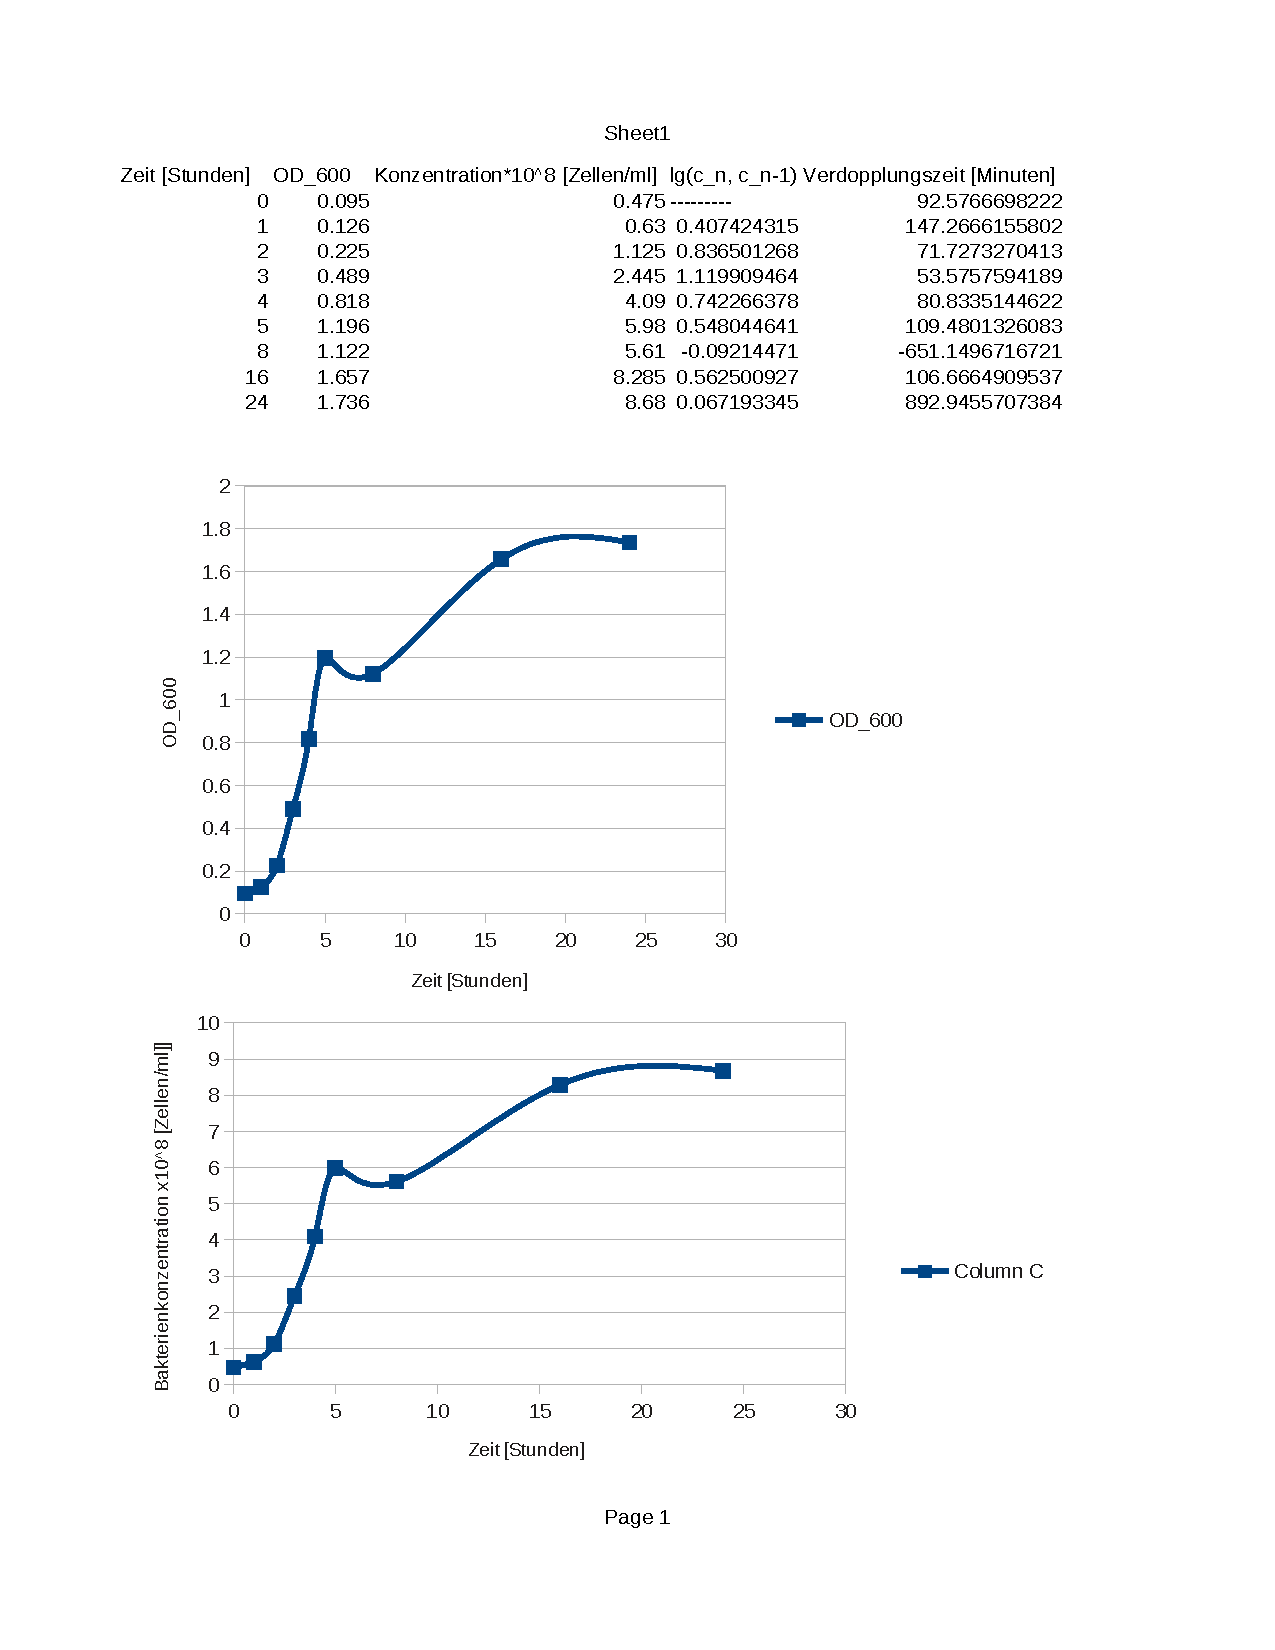
\includegraphics[scale=0.9]{OD600.pdf}\newpage
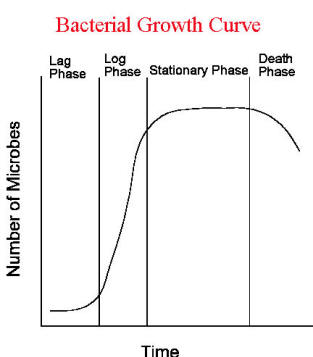
\includegraphics[scale=0.7]{bacterial growth curve.jpg}

\subsection{Diskussion}
Man sieht, dass beide Graphen einen identischen Steigungsverlauf besitzen, da $OD_{600}$ und die Bakteriendichte ja proportional sind. Die meisten Daten wurden in der Zeit 0 bis 8 generiert, allerdings muss ein Zeitraum bis über 24 Stunden hinaus betrachtet werden, damit ein Diagramm entsteht, das alle Phasen der Entwicklung der Kultur beinhaltet. Daher wirkt der Bereich der ersten 8 Stunden etwas gestaucht. Die Lag-Phase lässt sich dennoch innerhalb der ersten Stunde erkennen, zwischen dem ersten und zweiten Messpunkt. Zwischen dem zweiten und sechsten Messpunkt fand eindeutig die Log-Phase statt, der exponentielle Anstieg ist deutlich zu erkennen. Die restliche drei Messpunkte waren gegeben und nicht von uns im Rahmen des Versuchs experimentell bestimmt worden. Dabei beschreibt der siebte Messpunkt den $OD_{600}$ nach 8 Stunden. Da dieser, wie gesagt, mit innerhalb eines anderen Versuchs ermittelt worden ist, ist es nicht verwunderlich, dass das Wachstum plötzlich sinkt und die Konzentration sogar sinkt. Das kommt daher, dass zB in unserer Kultur mehr Bakterien zu Beginn waren, als in dem Versuch, der die restlichen drei Messwerte lieferte. Nichtsdestotrotz sieht man, wie nach spätestens 9-10 Stunden das Wachstum nachlässt und die stationäre Phase erreicht wird. Nun sterben bereits fast so viele Bakterien, wie neu durch Teilung entstehen können. Nach ca. 21 Stunden ist der absolute Höhepunkt der Bakterienkonzentration erreicht, nun sind die Nährstoffe fast erschöpft, und die toxischen Stoffwechselendprodukte haben sich derart angehäuft, dass nun viel mehr Bakterien sterben, als neue nachkommen, die Death Phase ist erreicht. Betrachet man einen Musterverlauf [2], so lassen sich eindeutige Zusammenhänge bezüglich der vier Phasen erkennen.\newline
Die Verdopplungszeit errechnet sich aus dem Verhältnis aufeinanderfolgender Bakterien konzentrationen. Nimmt man davon den Zweier Logarithmus und multipliziert den Kehrwert mit 60, so erhält man die aktuelle Verdopplungszeit. Die durchschnittliche Verdopplungszeit während der Log-Phase liegt hierbei bei ca. 93 Minuten, also eineinhalb Stunden. Während des Versuchs von ca. 5 Stunden fanden als ungefähr drei eindrittel Verdopplungszeiten statt, als hat sich die Bakterienkultur während der Log Phase $2^{3,3} = 10$ verzehnfacht. Dies sieht man auch im Diagramm: während der ersten 5 Stunden stieg die Anzahl an Bakterien von ca. 50 Millionen auf 600 Millionen an.

\section{Versuch 2: Transformation von Bakterien}
\subsection{Einleitung}
Wie man im ersten Versuch eindrucksvoll sehen konnte, können sich Bakterien innerhalb fünf Stunden verzehnfachen. Da bei jeder Teilung eine praktisch identische Kopie der Ausgangszelle entsteht, macht diese Tatsache Bakterien attraktiv für die Vervielfachung von zB genomischen Materials. Da Prokaryonten 
\subsection{Material, Methoden, Durchführung}
\subsection{Ergebnisse}
\subsection{Diskussion}

\section{Externe Quellen}
\begin{itemize}
\item $[1]$ http://en.wikipedia.org/wiki/Orange\_\%28colour\%29
\item $[2]$ http://www.bioc.rice.edu/bios576/nih\_bioreactor/NDL\_Bioreactor\%20Page.htm
\end{itemize}
\end{document}